\subsection{Netzwerk}
\label{subsec:netzwerk}

Aufgrund der vielen Komponenten, Funktionen und den möglichen Erweiterungen des \gls{go1} ist eine robuste interne Kommunikation nötig.
Die interne Kommunikationsstruktur des Roboters baut großenteils auf Netzwerkstandards wie \emph{Ethernet} und \emph{Wi-Fi} auf,
setzt besonders in der Konnektivität mit externen Komponenten jedoch zusätzlich auf weitere Standards wie \emph{Bluetooth} und \emph{\gls{wwan}}.

Das folgende Kapitel erläutert die vorhandene Kommunikation der internen und externen Komponenten des \gls{go1} und analysiert diese
auf ihre Stärken und Schwächen.
Zudem soll die Methodik der Analyse des Netzwerks und mögliche Problemfeststellungen und -behebungen festgehalten werden.

\subsubsection{Überblick}
\label{subsubsec:netzwerk_ueberblick}

Abbildung~\ref{fig:netzwerk_ueberblick} gilt als Referenz für die folgenden Ausführungen.
Zentrale Einheit der Kommunikation sind der verbaute Ethernet Switch und
der intern verbaute \emph{Raspberry Pi}.
Wie auf Abbildung~\ref{fig:netzwerk_ueberblick} zu erkennen ist, sind alle fünf Recheneinheiten -
der Raspberry Pi, die \gls{mcu}, die beiden NVIDIA Jetson Nanos und der Jetson Xavier NX -
per \emph{Ethernet} mit dem Switch verbunden.
Auch der extern zugängliche Ethernet-Port auf dem Rücken des Roboters ist mit dem Switch verbunden.

\begin{figure}[h]
    \frame{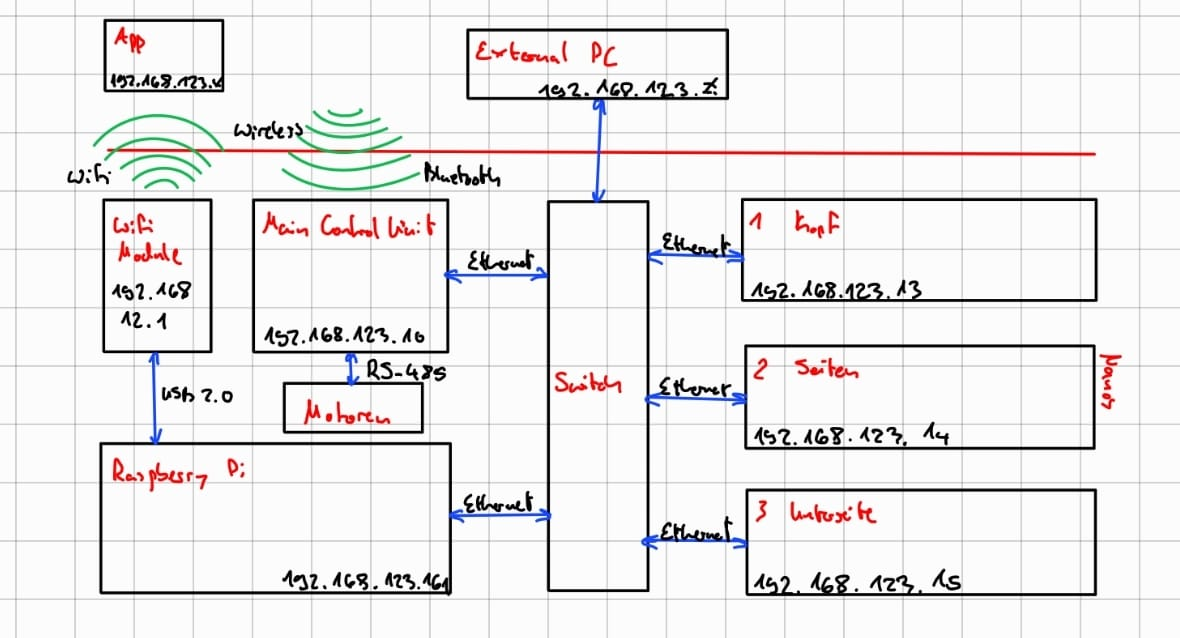
\includegraphics[width=\linewidth]{img/netzwerk/netzwerk_ueberblick}}
    \caption{Überblick über Netzwerkkonfiguration}\label{fig:netzwerk_ueberblick}
\end{figure}

Alle geswitchten Komponenten des Netzwerks sind im \texttt{192.168.123.0/24}-Netzwerk registriert.
Dabei ist die Verteilung der \gls{ip}-Adressen folgendermaßen vorkonfiguriert:
\begin{itemize}
    \item \textbf{\gls{mcu}:} \texttt{192.168.123.10}
    \item \textbf{Raspberry Pi:} \texttt{192.168.123.161}
    \item \textbf{NVIDIA Jetson Nanos:}
    \begin{enumerate}
        \item Kopf: \texttt{192.168.123.13}
        \item Seiten: \texttt{192.168.123.14}
    \end{enumerate}
    \item \textbf{NVIDIA Jetson Xavier NX:} \texttt{192.168.123.15}
\end{itemize}
Dem Endgerät, das am externen Ethernet-Port an der Oberseite des Roboters angesteckt werden kann,
muss eine statische \gls{ip}-Adresse im Bereich \texttt{192.168.123.0/24} vergeben werden, die nicht bereits von einem der oben genannten
Geräten verwendet wird.

Der Raspberry Pi hat zusätzlich zu seiner physischen Verbindung zum Switch und der \texttt{192.168.123.161}-\gls{ip}-Addresse
noch ein \gls{wlan} Modul verbaut, mit welchem er das Netz \texttt{192.168.12.0/24} publiziert.
Dieses Netz wird ab Werk für die Verbindung der App mit dem System benötigt.
Des Weiteren kann dieses Netz genutzt werden, um eine kabellose Verbindung mit dem Gesamtsystem
des Roboters herzustellen.

\subsubsection{Gekabelte Verbindung}

Wie bereits in Kapitel \ref{subsubsec:recheneinheiten} angerissen, besitzt der \gls{go1} auf der Oberseite des Rumpfes
eine RJ-45 Schnittstelle zur physischen Verbindung mit den Recheneinheiten.
Nachdem eine gekabelte Verbindung hergestellt wurde, muss auf der verbundenen Einheit eine statische \gls{ip} Adresse
konfiguriert werden, die nicht bereits von einer der verbauten Komponenten belegt ist.
Im Rahmen dieser Arbeit wird stets die \gls{ip} Adresse \texttt{192.168.123.51} angegeben.
Vergeben sind lediglich die Adressen, die im Überblick bereits gelistet wurden.
Ist die statische Adresse konfiguriert, können nun alle Systeme, bei denen \gls{ssh} aktiviert ist, erreicht werden.
Zu beachten ist lediglich, dass das Netzwerk nur ein geswitchtes Netzwerk ist, kein geroutetes.
Die interne Kommunikation muss also über Routen auf den einzelnen Recheneinheiten konfiguriert werden.
Ein Beispiel hierfür ist im folgenden Paragrafen zum Thema \emph{kabellose Verbindung} aufgeführt.

\subsubsection{Kabellose Verbindung}

Zu kabellosen Verbindung mit dem Netzwerk des \gls{go1} ist im Gegensatz zur gekabelten Verbindung keine statische \gls{ip}
Adresskonfiguration nötig.
Es muss sich lediglich mit dem \gls{wlan} Access Point verbunden werden, den der Raspberry Pi nach Systemstart aufspannt.
Die genaue Konfiguration dessen ist in Kapitel \ref{subsubsec:lokales-netzwerk} dokumentiert.

Nach Start des Roboters wird ein Access Point mit der Seriennummer des verwendeten \gls{go1} als \gls{ssid} aufgespannt.
Das Standardpasswort zur Verbindung ist \texttt{00000000}.
Die \gls{ip} Konfiguration des Hosts wird dann über \gls{dhcp} geregelt.
Der Access Point hat die Addresse \texttt{192.168.12.1}, weshalb dem Host auch eine Adresse im Netzwerk
\texttt{192.168.12.0/24} vergeben wird.

Um die interne Kommunikation des Pis mit dem Rest des Netzwerks besser nachvollziehen zu können, können die Forwarding-Regeln
und die \gls{ip} Routen des Systems ausgegeben werden.

\begin{lstlisting}[language=Bash]
pi@raspberrypi:~ $ cat /proc/sys/net/ipv4/ip_forward
1 # IP-Forwarding aktiviert
pi@raspberrypi:~ $ cat /etc/sysctl.conf | grep ip_forward
net.ipv4.ip_forward=1 # Dauerhafte Aktivierung des Forwarding
pi@raspberrypi:~ $ sudo iptables -L
[...]
Chain FORWARD (policy ACCEPT)
target     prot opt source               destination
ACCEPT     all  --  anywhere             anywhere
ACCEPT     all  --  anywhere             anywhere
[...]
\end{lstlisting}

\noindent Zu erkennen ist, dass das System alle Forwardingversuche zulässt.
Des Weiteren müssen für Kommunikation des \texttt{192.168.12.0/24} Netzes mit den Hosts im \texttt{192.168.123.0/24} Netz
die Routen auf dem Pi geprüft werden.

\begin{lstlisting}[language=Bash]
pi@raspberrypi:~ $ ip route | grep default
[...]
default via 192.168.123.1 dev eth0 src 192.168.123.161 metric 202
default via 192.168.12.1 dev wlan1 src 192.168.12.1 metric 305
[...]
\end{lstlisting}

\noindent Zu erkennen ist, dass die Standardroute aller Anfragen an das Gateway im Netz \texttt{..12.0/24} über das
Interface \texttt{wlan1} geleitet werden, worüber sie dann an den verbundenen Host kommen.
Umgekehrt werden alle Nachrichten des Host an das Netz \texttt{..123.0/24} über das Ethernet Interface \texttt{eth0}
geleitet, dass als Gateway fungiert und die Pakete an die Empfänger direkt weiterleitet, da diese über den Switch ohne
weitere Gateways erreichbar sind.

Auf den verbundenen NVIDIA Jetsons ist hingegen nur eine Standardroute definiert.

\begin{lstlisting}[language=Bash]
unitree@unitree-desktop:~$ ip route | grep default
default via 192.168.123.161 dev eth0
default via 192.168.123.1 dev eth0 onlink
\end{lstlisting}

\noindent Hier fungiert jeweils das Ethernet Interface \texttt{eth0} als Gateway und leitet alle unbekannten Adressen,
beispielsweise die des Netzes \texttt{..12.0/24}, über dieses Interface an die Adresse \texttt{192.168.123.161}, was
die Adresse des Ethernet Interfaces des Raspberry Pis ist.

\subsubsection{Weitere Netzwerk Funktionen}

Innerhalb des Raspberry Pis sind neben den Interfaces \texttt{eth0} und \texttt{wlan1} noch weitere Netzkarten verbaut.
Diese können beispielsweise genutzt werden, um den Pi mit einem \gls{wlan} Access Point zu verbinden oder ihn in ein
Mobilfunknetz einzuwählen.
Diese Funktionen werden genauer in den Kapiteln \ref{subsubsec:wifi} und \ref{subsubsec:gsm} erläutert.



